\section{\uppercase{Выполнение программы}}

Поскольку система распространяется в виде исходных кодов, необходимо сначала собрать все необходимые контейнеры. Это не требуется для пользователей веб-интерфейса, но обязательно для запуска серверной части и для загрузки индексов в систему.

\begin{lstlisting}
git clone https://github.com/iliakonnov/shatterbird.git
cd shatterbird
docker compose build --profile build
\end{lstlisting}

Это соберет следующие Docker-образы:
\begin{enumerate}
    \item shatterbird-backend
    \item shatterbird-cli
    \item shatterbird-frontend
    \item shatterbird-indexer
\end{enumerate}

\subsection{Запуск серверной части}

После этого можно запустить серверную часть одной командой:
\begin{lstlisting}
docker compose up
\end{lstlisting}

При этом будут автоматически запущены база данных, бекенд, а также веб-сервер, обеспечивающий доступ к пользовательской части. Также будет создана сеть с названием \texttt{shatterbird\_back}, в которой доступна база данных.

\subsection{Использование инструмента индексации}

Индексация репозитория происходит в два этапа.

Сначала необходимо загрузить данные Git-репозитория в базу данных:

\noindent\begin{minipage}[t]{0.45\textwidth}
\begin{lstlisting}
docker run                            \
    --rm                              \
    --env RUST_LOG=info               \
    --network shatterbird_back        \
    --volume ./:/repo:ro              \
    shatterbird-indexer               \
    --db-url mongodb://mongo:27017/db \
    git                               \
    --root /repo                      \
    --max-depth 3
\end{lstlisting}
\end{minipage}\hfil\begin{minipage}[t]{0.50\textwidth}\footnotesize\setlength{\baselineskip}{14.7pt}
\vspace{16pt}
— удалить контейнер после завершения \\
\\
— использовать ту же сеть, в которой запущена БД \\
— смонтировать текущую директорию внутрь контейнера \\
— имя собранного контейнера \\
— строка подключения к базе данных \\
— указывает на загрузку данных Git-репозитория \\
— директория репозитория внутри контейнера \\
— максимальная глубина загрузки родительских коммитов
\end{minipage}

Эта команда загрузит данные репозитория из текущей директории в базу данных. Будет загружен текущий коммит, а также все его родительские, если расстояние до них не превышает 3. При этом обязательно требуется, чтобы была запущена база данных.

А результате работы будет выведен идентифкатор загруженного объекта в базе данных:
\begin{lstlisting}
commits[6640ae26d07021dfb873cb20]
\end{lstlisting}

Затем можно загрузить данные индекса из результата работы LSIF-совместимого индексатора:
\begin{lstlisting}
docker run                                         \
    --rm                                           \
    --env RUST_LOG=info                            \
    --network shatterbird_back                     \
    --volume ./index.lsif.json:/index.lsif.json:ro \
    shatterbird-indexer                            \
    --db-url mongodb://mongo:27017/db              \
    lsif                                           \
    --input /index.lsif.json                       \
    --save                                         \
    --roots /Documents/shatterbird=6640ae26d07021dfb873cb20
\end{lstlisting}

При этом в программу передаётся следующая информация:
\begin{itemize}
    \item Имя файла, содержащего результат индексации. В примере используется \texttt{index.lsif.json}.
    \item Указание, что в результатах индексации путь «\texttt{/Documents/shatterbird}» соответствует загруженному в предыдущем этапе коммиту «\texttt{6640ae26d07021dfb873cb20}». Параметр командной строки «\texttt{-\/-roots}» может указываться несколько раз при использовании нескольких репозиториев в рамках одного индексируемого проекта.
\end{itemize}

Опциональный параметр \texttt{-\/-save} указывает на необходимость сохранить полученные данные в базу данных.

\subsection{Использование пользовательского интерфейса}

Для начала использования, достаточно открыть адрес веб-сервера в браузере. После этого в левой части экрана будет возможно просматривать список проиндексированных коммитов, а также просматривать список файлов в каждой доступной версии репозитория. В правой части отображается содержимое выбранного файла.

\begin{figure}[H]
    \centering
    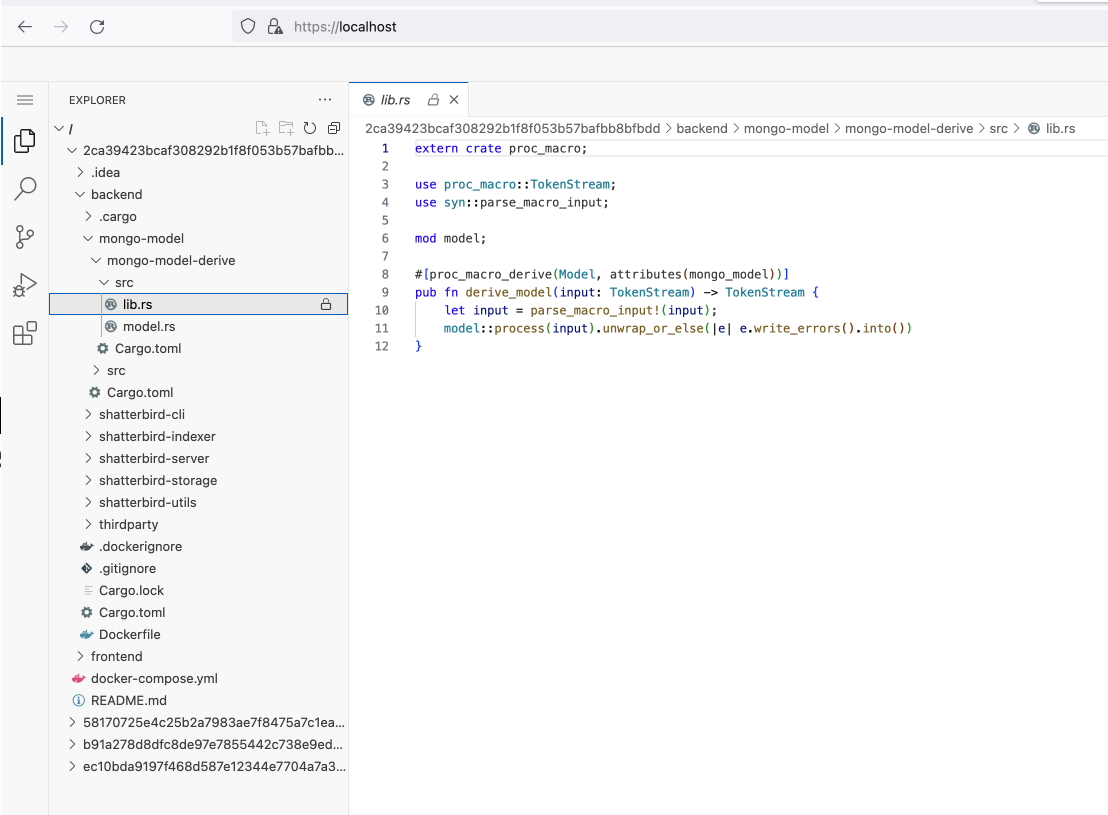
\includegraphics[width=\textwidth]{figures/intro.png}
    \caption{Вид пользовательского интерфейса}
\end{figure}

При клике правой кнопкой мыши по содержимому файла, появляется контекстное меню, предоставляющее следующие функции:

\begin{itemize}
    \item «Go to definiton» — перейти к определению символа под курсором.
    \item «Go to references» — найти все использования символа под курсором.
\end{itemize}

\begin{figure}[H]
    \centering
    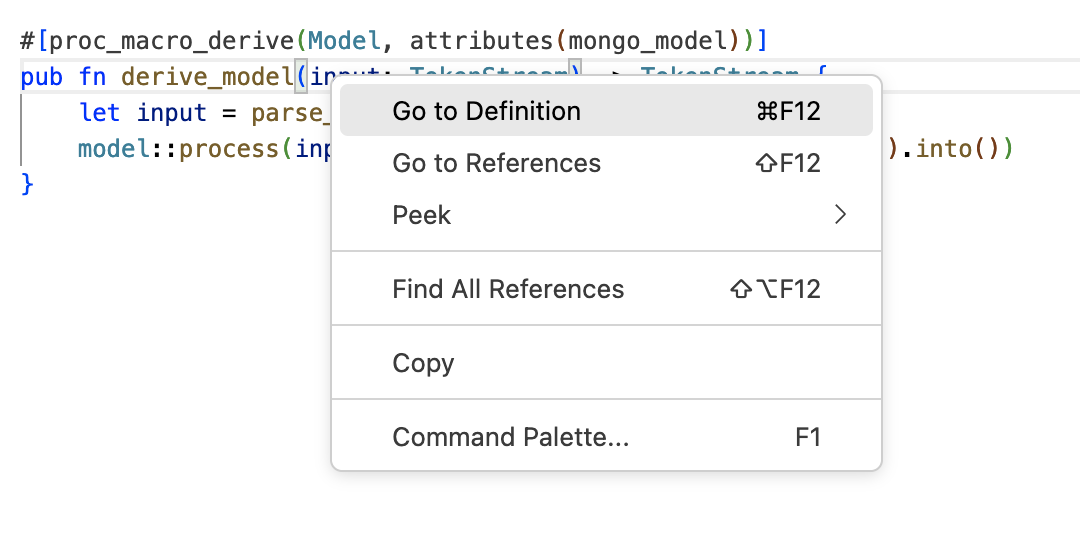
\includegraphics[width=0.5\textwidth]{figures/menu.png}
    \caption{Контекстное меню}
\end{figure}

\clearpage